\chapter{Az impulzusmomentum}

 \section{Mechanika}
  
  \subsection{Egyetlen tömegpont esete}
 
   Az impulzusmomentum (perdület) definíciója: 
   \eq{
    \Lv=\rv\times\pv=m\rv\times\dot\rv.
   }
   Hengerkoordinátákban kifejtve: $\Lv=m\cdot(r\ev_r)\times(\dot{r}\ev_r+r\dot{\phi}\ev_\varphi)=mr^2\dot{\varphi}\cdot\ev_z$. Centrális erőtérben a tömegpont perdülete állandó. Legyen $\Fv=F(r)\frac{\rv}{r}=F(r)\ev_r$, akkor $\dot{\Lv}=\dot{\rv}\times\pv+\rv\times\dot\pv=0+0=0$, hiszen $\dot\rv\parallel \vv$ és $\dot\pv=\Fv\parallel\rv$.
   
   Számítsuk ki az $\Lv^2$-et is:
   \al{
    \Lv^2
     =\ep_{ijk}x_jp_k\ep_{ilm}x_lp_m
     =\big(\delta_{jl}\delta_{km}-\delta_{jm}\delta_{kl}\big)x_jp_kx_lp_m
     =\rv^2\pv^2-(\rv\pv)^2.
   }
   
   A forgatónyomaték definíciója:
   \eq{
    \Mv=\rv\times\Fv.
   }
   Az impulzusmomentum csak adott koordináta-rendszerben értelmezett, minden esetben meg kell adni, hogy milyen pontra vonatkoztatjuk a perdületet. A forgatónyomaték is ehhez hasonló, ott is egy $\Fv$ erő adott pontra vonatkoztatott forgatónyomatékát lehet csak értelmezni.
   
   Számítsuk ki a tömegpont mozgási energiáját szintén hengerkoordináta-rendszerben:
   \al{
    E_\text{kin}
     &=\frac 12 m\vv^2
      =\frac 12 m\big(\dot{r}\ev_r+r\dot{\varphi}\ev_\varphi\big)^2
      =\frac 12 m\dot{r}^2+\frac 12 mr^2\dot{\varphi}^2
      =\frac 12 m\dot{r}^2+\frac{L^2}{2mr^2}.
   }
   Itt bevezethetjük a radiális impulzust: $\pv_r=m\dot r\ev_r$, illetve a második tag a forgásból (keringésből) adódó energiajárulék. 
  
  \subsection{Pontrendszerek}\label{ss6:pontrendszerek}
   
   Térjünk át a pontrendszerek esetére. Legyen egy $N$ pontból álló rendszerünk. Ennek perdülete:
   \eq{
    \Lv=\suml{i=1}{N}\Lv_i=\suml{i=1}{N}\rv_i\times\pv_i=\suml{i=1}{N}m_i\rv_i\times\dot\rv_i.
   }
   Számítsuk ki a perdület időbeli megváltozását:
   \eq{
    \dot\Lv
     =\suml{i=1}{N}\rv_i\times\dot\pv_i
     =\suml{i=1}{N}\rv_i\times\Fv_i
     =\suml{i=1}{N}\rv_i\times\left(\suml{j=1(\neq i)}{N}\Fv_{ji}+\Fv_{\text{k},i}\right),
   }
   ahol az $i$-edik tömegpontra ható erőt felbontottuk egy külső $\Fv_{\text{k},i}$ és a belső erők eredőjére. A külső erők járuléka egy külső forgatónyomaték: $\Mv_\text{k}=\suml{i=1}{N}\rv_i\times\Fv_{\text{k},i}$. A belső erők járulékánál kihasználjuk a III. Newton-törvényt:
   \al{
    \dot{\Lv}
     &=\Mv_\text{k}+\suml{i\neq j}{N}\rv_i\times\Fv_{ji}
      =\Mv_\text{k}+\frac 12\suml{i\neq j}{N}\big(\rv_i\times\Fv_{ji}+\rv_j\times\Fv_{ij}\big)
      =\Mv_\text{k}+\frac 12\suml{i\neq j}{N}\big(\rv_i\times\Fv_{ji}-\rv_j\times\Fv_{ji}\big)\\
     &=\Mv_\text{k}+\frac 12\suml{i\neq j}{N}\big(\rv_i-\rv_j\big)\times\Fv_{ji}.
   }
   A második tag pl. centrális erőkre nulla. Ha a rendszerre ható forgatónyomaték nulla, akkor a rendszer teljes impulzusmomentuma megmarad. 
  
  \subsection{Pontrendszerek tömegközépponti koordináta-rendszerben}
   
   Érdemes bevezetni a tömegközéppont fogalmát:
   \eq{
    \Rv_\text{tkp}=\frac{\suml{i=1}{N}m_i\rv_i}{\suml{i=1}{N}m_i}=\frac{\suml{i=1}{N}m_i\rv_i}{M}.
   }
   Ez a mennyiség jól definiált, mert koordinátatranszformációkra vektorként viselkedik. Toljuk el az origót $\rv_0$-lal, akkor a tömegközéppont $\bar{\Rv}_\text{tkp}={\Rv}_\text{tkp}+\rv_0$ lesz. Deriváljuk idő szerint a tömegközéppontot definiáló egyenletet:
   \eq{
    M\dot{\Rv}_\text{tkp}=\suml{i=1}{N}m_i\dot\rv_i=\Pv_\text{tkp},
   }
   ezt még egyszer deriválva: 
   \al{
    M\ddot{\Rv}_\text{tkp}
     &=\dot\Pv_\text{tkp}
      =\suml{i=1}{N}m_i\ddot\rv
      =\suml{i=1}{N}\Fv_i
      =\suml{i=1}{N}\left(\suml{j=1(\neq i)}{N}\Fv_{ji}+\Fv_{\text{k},i}\right)
      =\underbrace{\suml{i\neq j}{N}\Fv_{ji}}_{=0}+\suml{i=1}{N}\Fv_{\text{k},i}
      =\Fv_\text{k}.
   }
   Tehát a Newton-egyenlet igaz egy pontrendszerre olyan értelemben, hogy annak tömegközéppontjának mozgását a külső erők eredője határozza meg. Ha a külső erők eredője nulla, akkor a tömegközéppont egyenesvonalú egyenletes mozgást végez, ez a tömegközéppont-megmaradás tétele. 
   
   Számoljuk ki a fenti mennyiségeket a tömegközépponti koordinátákat használva: $\rv_i=\bar\rv_i+\Rv_\text{tkp}$, ahol $\bar\rv_i$ a tömegközéppontból mért helyvektor. Az impulzus:
   \al{
    \Pv
     =\suml{i=1}{N}m_i\dot\rv_i
     =\suml{i=1}{N}m_i\big(\dot{\bar{\rv}}_i+\dot\Rv_\text{tkp}\big)
     =M\dot\Rv_\text{tkp}+\suml{i=1}{N}m_i\dot{\bar{\rv}}_i.
   }
   Az impulzusmomentum:
   \al{
    \Lv
    &=\suml{i=1}{N}\rv_i\times\pv_i
     =\suml{i=1}{N}\big(\bar\rv_i+\Rv_\text{tkp}\big)\times\big(\bar\pv_i+m_i\dot\Rv_\text{tkp}\big)\\
    &=\suml{i=1}{N}\bar\rv_i\times\bar\pv_i
      +\underbrace{\left(\suml{i=1}{N}m_i\bar\rv_i\right)}_{=0}\times\dot\Rv_\text{tkp}
      +\Rv_\text{tkp}\times\underbrace{\left(\suml{i=1}{N}\bar\pv_i\right)}_{=0}
      +\underbrace{\Rv_\text{tkp}\times\left(\suml{i=1}{N}m_i\right)\dot\Rv_\text{tkp}}_{=\Rv_\text{tkp}\times\Pv_\text{tkp}}\\
    &=\Rv_\text{tkp}\times\Pv_\text{tkp}+\suml{i=1}{N}\bar\rv_i\times\bar\pv_i.
   }
   A perdület tehát egyenlő a tömegközéppont által képviselt perdület és az egyes tömegpontok tömegközéppontra viszonyított perdület összegével.
   
   Az impulzusmomentum mozgásegyenlete a tömegközépponti koordináták használatával:
   \al{
    \dot\Lv
     &=\der{}{t}\left(\Rv_\text{tkp}\times\Pv_\text{tkp}+\suml{i=1}{N}\bar\rv_i\times\bar\pv_i\right)
      =\underbrace{\dot\Rv_\text{tkp}\times\Pv}_{\dot\Rv_\text{tkp}\parallel\Pv}
       +\Rv_\text{tkp}\times\dot\Pv
       +\suml{i=1}{N}\underbrace{\dot{\bar{\rv}}_i\times\bar\pv_i}_{\dot{\bar{\rv}}_i\parallel\bar\pv_i}
       +\suml{i=1}{N}\bar\rv_i\times\dot{\bar{\pv}}_i\\
     &=0+\Rv_\text{tkp}\times\Fv_\text{k}
       +0+\suml{i=1}{N}\bar\rv_i\times\dot{\bar{\pv}}_i.
   }
   Itt $\pv_i=m_i\dot\rv_i={\bar\pv}_i+m_i\dot{\Rv}_\text{tkp}$, így ${\bar\pv}_i=\pv_i-m_i\dot{\Rv}_\text{tkp}=\pv_i-\frac{m_i}{M}\Pv_\text{tkp}$.
   \al{
    \dot\Lv
     &=\Rv_\text{tkp}\times\Fv_\text{k}
       +\suml{i=1}{N}\bar\rv_i\times\left(\dot\pv_i-\frac{m_i}{M}\dot\Pv\right)
      =\Rv_\text{tkp}\times\Fv_\text{k}
       +\suml{i=1}{N}\bar\rv_i\times\dot\pv_i
       -\frac{1}{M}\underbrace{\left(\suml{i=1}{N}m_i\bar\rv_i\right)}_{=0}\times\dot\Pv_\text{tkp}\\
     &=\Rv_\text{tkp}\times\Fv_\text{k}
       +\suml{i=1}{N}\bar\rv_i\times\left(\Fv_{\text{k},i}+\suml{j=1(\neq i)}{N}\Fv_{ji}\right),
   }
   ahol centrális erőket feltételezve:
   \eq{
    \dot\Lv
     =\Rv_\text{tkp}\times\Fv_\text{k}
       +\suml{i=1}{N}\bar\rv_i\times\Fv_{\text{k},i}.
   }
   Ez szintén értelmezhető úgy, hogy a pontrendszerre ható külső erők forgatónyomatéka egyenlő a külső rendszerben tömegközéppontra ható, és az egyes tömegpontokra ható a tömegközéppontra vonatkoztatott forgatónyomaték összegével.
   
   Írjuk fel az energiát is ebben a felbontásban:
   \al{
    E_\text{kin}
     &=\frac{1}{2}\suml{i=1}{N}m_i\dot{\rv}_i^2
      =\frac{1}{2}\suml{i=1}{N}m_i\big(\dot{\bar\rv}_i+\dot\Rv_\text{tkp}\big)^2
      =\frac{1}{2}\suml{i=1}{N}m_i\big(\dot{\bar\rv}_i\big)^2
       +\frac{1}{2}\suml{i=1}{N}m_i\big(\dot\Rv_\text{tkp}\big)^2
       +\dot\Rv_\text{tkp}\underbrace{\suml{i=1}{N}m_i\dot{\bar\rv}_i}_{=0}\\
     &=\frac{1}{2}\suml{i=1}{N}m_i\big(\dot{\bar\rv}_i\big)^2
       +\frac{1}{2}M\big(\dot\Rv_\text{tkp}\big)^2,
   }
   ami megegyezik a tömegközéppont mozgási energiájának és a tömegközépponti koordináta-rendszerben az egyes tömegpontok mozgási energiájának összegével. 
   
   \subsection{Merev testek, forgás, tehetetlenségi nyomaték}
   
   Merev test az olyan pontrendszer, ahol $\{\bar\rv_i\}$ $\forall i$-re rögzített, az a mozgás során állandó. Egy ilyen test mozgása haladó- és forgómozgásból áll (Euler-tétel). Minden tömegpont sebességét felírhatjuk a 
   \eq{
    \vv_i=\vv_0+\omv\times(\rv_i-\rv_0)
   }
   felbontásban, ahol $\vv_0$ és $\rv_0$ a merev test egy kitüntetett pontjának haladó mozgását, míg $\omv$ az ez a pont körüli forgómozgást írja le. Az impulzusmomentum:
   \al{
    \Lv
     &=\suml{i=1}{N}m_i\rv_i\times\vv_i
      =\suml{i=1}{N}m_i\rv_i\times\big(\vv_0+\omv\times(\rv_i-\rv_0)\big)
      =M\Rv\times\vv_0+\suml{i=1}{N}m_i\rv_i\times\big(\omv\times(\rv_i-\rv_0)\big).
   }
   Az első tag a test haladásához kapcsolódó impulzusmomentum. Ez eltűnik, ha az origó a test tömegközéppontjában van, vagy ha a test nem végez haladómozgást. 
   
   Legyen a kitüntetett pont az origó, így $\rv_0=0$. Fejtsük ki a második tagot:
   \al{
    \Big[m_i\rv_i\times\big(\omv\times\rv_i\big)\Big]_j
     &=m_i\ep_{jkl}\big[\rv_i\big]_k\ep_{lmn}[\omv]_m\big[\rv_i\big]_n
      =m_i\Big(\delta_{jm}\delta_{kn}-\delta_{jn}\delta_{km}\Big)\big[\rv_i\big]_k[\omv]_m\big[\rv_i\big]_n\\
     &=m_i\Big([\omv]_jr_i^2-\big[\rv_i\big]_j[\omv]_m\big[\rv_i\big]_m\Big)
      =m_i\Big(\delta_{jm}r_i^2-\big[\rv_i\big]_j\big[\rv_i\big]_m\Big)[\omv]_m.
   }
   Ezzel az impulzusmomentum:
   \al{
    &\Lv=\mat\Theta\omv&
    &[\mat\Theta]_{jk}=\suml{i=1}{N}m_i\Big(\delta_{jk}r_i^2-\big[\rv_i\big]_j\big[\rv_i\big]_k\Big)&\\
     & & &\phantom{[\mat\Theta]_{jk}}=\begin{pmatrix}
       \suml{i=1}{N}m_i\big(y_i^2+z_i^2\big) & \suml{i=1}{N}m_i\big(-x_iy_i\big) & \suml{i=1}{N}m_i\big(-x_iz_i\big) \\
       \suml{i=1}{N}m_i\big(-x_iy_i\big) & \suml{i=1}{N}m_i\big(x_i^2+z_i^2\big) & \suml{i=1}{N}m_i\big(-y_iz_i\big) \\
       \suml{i=1}{N}m_i\big(-x_iz_i\big) & \suml{i=1}{N}m_i\big(-y_iz_i\big) & \suml{i=1}{N}m_i\big(x_i^2+y_i^2 \big)
      \end{pmatrix},&
   }
   ahol bevezettük a $\mat\Theta$ tehetetlenségi nyomatékot. Ennek alakja folytonos $\rho(\rv)$ tömegeloszlás esetén:
   \eq{
    [\mat\Theta]_{jk}=\intl{V}{}\drh\rho(\rv)\Big(\delta_{jk}r^2-\big[\rv\big]_j\big[\rv\big]_k\Big)
   }
   
   Kiszámítjuk a kinetikus energiát is:
   \al{
    E_\text{kin}
     &=\frac{1}{2}\suml{i=1}{N}m_i\dot{\rv}_i^2
      =\frac{1}{2}\suml{i=1}{N}m_i\big(\vv_0+\omv\times\rv_i\big)^2\\
     &=\frac{1}{2}\suml{i=1}{N}m_i\vv_0^2
       +\vv_0\left(\omv\times\suml{i=1}{N}m_i\rv_i\right)
       +\frac{1}{2}\suml{i=1}{N}m_i\big(\omv\times\rv_i\big)^2.
   }
   Itt az első tag a test transzlációs mozgásához kapcsolódó kinetikus energia. A második tag a tömegközépponti koordináta-rendszerben eltűnik, míg a harmadik tag a forgómozgáshoz kapcsolódó kinetikus energia. Ez kifejtve:
   \al{
    m_i\big(\omv\times\rv_i\big)^2
     &=m_i(\omv\times\rv_i)\cdot(\omv\times\rv_i)
      =\big(m_i\rv_i\times(\omv\times\rv_i)\big)\cdot\omv,
   }
   \eq{
    E_\text{kin}
     =\frac{1}{2}M\vv_0^2+\frac 12\Lv\omv=\frac{1}{2}M\vv_0^2+\frac 12\omv^T\mat\Theta\omv.
   }
   
   Ha a forgástengely iránya adott, akkor a forgási energia: $E_\text{forg}=\frac 12 I\omega^2$, ahol $I$ az adott tengelyre vonatkozó tehetetlenségi nyomaték:
   \al{
    I&=\nv\mat\Theta\nv
      =[\nv]_j[\mat\Theta]_{jk}[\nv]_k
      =[\nv]_j\suml{i=1}{N}m_i\Big(\delta_{jk}r_i^2-\big[\rv_i\big]_j\big[\rv_i\big]_k\Big)[\nv]_k
      =\suml{i=1}{N}m_i\Big(n^2r_i^2-(\rv\nv)^2\Big)\\
     &=\suml{i=1}{N}m_i\big(\rv_{i,\perp}\big)^2,
   }
   ahol az $\rv_{i,\perp}$ az $i$-edik tömegpont forgástengelytől mért távolsága. 
   
   Nézzünk egy speciális esetet, amikor a forgástengely a tömegközépponton megy át. Kérdés, hogy mekkora lesz a forgatónyomaték, ha ezt a tengelyt eltoljuk a tömegközéppontból $\lv$-lel. A forgástengely iránya nem változik, csak annak helye. A Steiner-tétel:
   \al{
    \bar{I}
     &=\suml{i=1}{N}m_i\big(\rv_{i,\perp}-\lv\big)^2
      =\suml{i=1}{N}m_i\big(\rv_{i,\perp}\big)^2
       +2\lv\suml{i=1}{N}m_i\rv_{i,\perp}
       +\suml{i=1}{N}m_i\lv^2
     =I+M\lv^2.
   }
%    {\color{red} Esetleg írni lehetne még, hogy miért deviációs nyomatékok a $\mat\Theta$ offdiagonális elemei, talán a pörgettyűkről, nutáció, precesszió, az örök szenvedély\dots}
   
 \section{Elektrodinamika}
  
%    {\color{red} Hiányosság: írd bele azt is, hogy az origóban nem értelmezhetőek a terek, ott még egy dirac-delta töltés hiányzik, számoljuk is ki!!!}
  \subsection{A mágneses dipólmomentum}
  
  Definíciója (részletek a multipól sorfejtésnél \aref{eq:ss-11multipol}. fejezet): 
  \eq{
   \emv=\frac{1}{2}\intl{}{}\drh\rv\times\Jv(\rv).
  }
  Vezető hurok esetén ez:
  \al{
   m_i
    &=\frac{1}{2}\ep_{ijk}\intl{}{}\drh r_j J_k
     =\frac{I}{2}\oint\limits\dd s_k\, \ep_{ijk}r_j
     =\frac{I}{2}\intl{F}{}\dd f_k\, \ep_{kln}\partial_l\ep_{ijn}r_j
     =\frac{I}{2}\intl{F}{}\dd f_k\, 2
     =If_i,
  }
  vagyis $\emv=I\fv$. 
  
 \subsection{Kapcsolat a dipólmomentum és a perdület között}
  
  Legyen egy elektron, melyre alkalmazzuk az előző összefüggést. Ennek $\Jv(\rv)=-e\vv\delta\big(\rv-\rv_0(t)\big)$. Így
  \eq{
   \emv=-e\frac{1}{2}\intl{}{}\drh\rv\times\vv\delta\big(\rv-\rv_0(t)\big)
      =-e\frac{1}{2}\rv_0(t)\times \vv
      =-\frac{e}{2m}\Lv.
  }
  
  \subsection{Mágneses dipól tere}
  \Aref{ss:A04}. tételnél láttuk, hogy a kis áramhurok által létrehozott vektorpotenciál:
  \eq{
   \vect{A}(\vect{r})=\frac{\mu_0}{4\pi}\frac{\vect{m}\times\vect{r}}{\abs{\vect{r}}^{3}}.
  }
  A mágneses indukció:
  \al{
   B_i
    &=\ep_{ijk}\partial_jA_k
     =\ep_{ijk}\partial_j\frac{\mu_0}{4\pi}\frac{\ep_{kln}m_l r_n}{r^3}
     =\frac{\mu_0}{4\pi}\big(\delta_{il}\delta_{jn}-\delta_{in}\delta_{jl}\big)\partial_j\frac{m_l r_n}{r^3}\\
    &=\frac{\mu_0}{4\pi}\big(\delta_{il}\delta_{jn}-\delta_{in}\delta_{jl}\big)
      \left(\frac{m_l \delta_{jn}}{r^3}-3\frac{m_l r_nr_j}{r^5}\right)\\
     &=\frac{\mu_0}{4\pi}\frac{3m_ir^2-3m_i r^2-m_ir^2+3r_i(\vect{m}\rv)}{r^5}
      =\frac{\mu_0}{4\pi}\frac{3r_i(\vect{m}\rv)-m_ir^2}{r^5}
  }
  
  \subsection{Statikus elektromos dipólusok és azok kölcsönhatása}\label{ss:A06-dipol}
   
   Legyen a $+\frac{\av}{2}$ és a $-\frac{\av}{2}$-ben egy $+q$ és egy $-q$ töltés. Ezek elektromos potenciálja, ha $a\to0$:
   \al{
    \phi(\rv)
     &=\frac{q}{4\pi\ep_0}\left[\frac{1}{\abs{\rv-\frac{\av}{2}}}-\frac{1}{\abs{\rv+\frac{\av}{2}}}\right]
      \approx\frac{1}{4\pi\ep_0}\frac{q\av\rv}{\abs{\rv}^3}
      =\frac{1}{4\pi\ep_0}\frac{\pv\rv}{\abs{\rv}^3}
      =-\frac{1}{4\pi\ep_0}\pv\grad\frac{1}{\abs{\rv}},
   }
   ahol $\pv=q\av$ a dipólus erőssége. Az elektromos térerősség:
   \eq{
    \Ev(\rv)
     =-\grad{\phi(\rv)}
     =-\frac{1}{4\pi\ep_0}\grad\frac{\pv\rv}{\abs{\rv}^3}
     =\frac{1}{4\pi\ep_0}\frac{3\rv(\pv\rv)-\pv r^2}{\abs{\rv}^5}.
   }
   
   Két ilyen dipólus kölcsönhatási energiája: 
   \al{
    U_{12}=-\pv_2\Ev_1=\frac{1}{4\pi\ep_0}\frac{\pv_1\pv_2 r^2-3(\pv_1\rv)(\pv_2\rv)}{\abs{\rv}^5}.
   }
   
   Illetve két ilyen dipól közötti erő:
   \eq{
    \Fv_{12}
     =-\grad{U_{12}}
     =-\grad\left(\frac{1}{4\pi\ep_0}\frac{\pv_1\pv_2 r^2-3(\pv_1\rv)(\pv_2\rv)}{\abs{\rv}^5}\right).
   }
   
  \subsection{Mágneses és elektromos dipól összehasonlítása}
   
   \begin{center}
    \begin{tabular}{r||c|c}
     Tulajdonság & Elektromos dipólmomentum & Mágneses dipólmomentum \\ \hline
      momentum nagysága & $\pv=q\av$ & $\emv=I\fv$ \\
      momentum meghatározása & $\pv=\intl{}{}\drh\rv\rho(\rv)$ & $\emv=\frac{1}{2}\intl{}{}\drh\rv\times\Jv(\rv)$ \\
      potenciál & $\phi(\rv)=\frac{1}{4\pi\ep_0}\frac{\pv\rv}{\abs{\rv}^3}$ & $\vect{A}(\vect{r})=\frac{\mu_0}{4\pi}\frac{\vect{m}\times\vect{r}}{\abs{\vect{r}}^{3}}$ \\
      tér & $\Ev(\rv)=\frac{1}{4\pi\ep_0}\frac{3\rv(\pv\rv)-\pv r^2}{\abs{\rv}^5}$ & $\Bv(\rv)=\frac{\mu_0}{4\pi}\frac{3\rv(\vect{m}\rv)-\emv r^2}{r^5}$ \\
      forgatónyomaték homogén térben & $\Mv=\pv\times\Ev$ & $\Mv=\emv\times\Bv$ \\
      energia külső térben & $U=-\pv\Ev$ & $U=-\emv\Bv$
    \end{tabular}
   \end{center}
   
   Az elektromos és a mágneses dipólus között különbség a közeltérben való szerkezetük. Az elektromos dipólban a két töltés között a térerősség iránya párhuzamos a külső térrel, míg a mágneses dipólnál a gyűrű közepén a tér ellentétesen mutat, mint a gyűrű mellett azon kívül.

   
 \section{Kvantummechanika}
  
  \subsection{Az impulzusmomentum operátora, algebrája}
  
   Az impulzusmomentum operátorát a klasszikus mechanikához hasonlóan definiáljuk itt is:
   \eq{
    \opLv=\oprv\times\oppv=\begin{pmatrix}
                            \op{y}\op{p}_z-\op{z}\op{p}_y\\
                            \op{z}\op{p}_x-\op{x}\op{p}_z\\
                            \op{x}\op{p}_y-\op{y}\op{p}_x
                           \end{pmatrix}.
   }
   Vizsgáljuk meg az $\opLv$ operátor komponenseinek kommutációs relációit:
   \al{
    [\op{L}_i,\op{L}_j]
     &=\ep_{ikl}\ep_{jmn}\big[\op{x}_k\op{p}_l,\op{x}_m\op{p}_n\big]\\
     &=\ep_{ikl}\ep_{jmn}\Big(
       \op{x}_k\op{x}_m\big[\op{p}_l,\op{p}_n\big]
      +\op{x}_k\big[\op{p}_l,\op{x}_m\big]\op{p}_n
      +\op{x}_m\big[\op{x}_k,\op{p}_n\big]\op{p}_l
      +\big[\op{x}_k,\op{x}_m\big]\op{p}_n\op{p}_l\Big)\\
     &=\frac{\hbar}{i}\ep_{ikl}\ep_{jmn}\Big(
       \delta_{lm}\op{x}_k\op{p}_n
      -\delta_{kn}\op{x}_m\op{p}_l\Big)
      =\frac{\hbar}{i}\Big(
       \ep_{ikl}\ep_{jln}\op{x}_k\op{p}_n
      -\ep_{inl}\ep_{jmn}\op{x}_m\op{p}_l\Big)\\
     &=\frac{\hbar}{i}\Big(
       \big(\delta_{ni}\delta_{kj}-\delta_{ij}\delta_{nk}\big)\op{x}_k\op{p}_n
      -\big(\delta_{mi}\delta_{lj}-\delta_{ij}\delta_{lm}\big)\op{x}_m\op{p}_l\Big)\\
     &=i\hbar\big(\op{x}_i\op{p}_j-\op{x}_j\op{p}_i\big)=i\hbar \ep_{ijk}\op{L}_k.
   }
   Ez átírható másik alakba:
   \al{
    \big[\opLv\times\opLv\big]_i
     &=\ep_{ijk}\op{L}_j\op{L}_k
      =\frac 12 \Big(\ep_{ijk}\op{L}_j\op{L}_k+\ep_{ikj}\op{L}_k\op{L}_j\Big)
      =\frac 12 \ep_{ijk}\Big(\op{L}_j\op{L}_k-\op{L}_k\op{L}_j\Big)\\
     &=\frac 12 \ep_{ijk}\Big[\op{L}_j\op{L}_k\big]
      =i\hbar\frac 12 \underbrace{\ep_{ijk}\ep_{jkl}}_{=2\delta_{il}}\op{L}_l
      =i\hbar\op{L}_i,
   }
   azaz
   \eq{
    \opLv\times\opLv=i\hbar\opLv.
   }
   
   Az $\op{L}^2$-tel azonban mindegyik felcserélhető:
   \al{
    \big[\op{L}^2,\op{L}_i\big]
     &=\big[\op{L}_j\op{L}_j,\op{L}_i\big]
      =\op{L}_j\big[\op{L}_j,\op{L}_i\big]+\big[\op{L}_j,\op{L}_i\big]\op{L}_j=i\hbar\ep_{jik}\big(\op{L}_j\op{L}_k+\op{L}_k\op{L}_j\big)=0,
   }
   hiszen egy szimmetrikus és egy antiszimmetrikus tag szorzata.
   
   Kiszámolhatjuk még a hely és az impulzus operátorával vett felcserélési relációit, ezek a következők lesznek:
   \al{
    &\big[\op{L}_i,\op{x}_j\big]=i\hbar\ep_{ijk}\op{x}_k&
    &\big[\op{L}_i,\op{x}_j^2\big]=0&
    &\big[\op{L}^2,\op{x}_j\big]=0&\\
    &\big[\op{L}_i,\op{p}_j\big]=i\hbar\ep_{ijk}\op{p}_k&
    &\big[\op{L}_i,\op{p}_j^2\big]=0&
    &\big[\op{L}^2,\op{p}_j\big]=0.&
   }
   
  \subsection{Radiális impulzus, $\oppv^2$ és $\opLv^2$ kapcsolata}
   
   A célunk, hogy az impulzus operátorának négyzetét fel tudjuk bontani egy radiális és egy szögektől függő komponensre. A szögektől függő rész az $\opLv^2$-tel lesz kapcsolatban, a radiális rész pedig egy új operátorral fejezhető ki, ez a radiális impulzus lesz. 
   
   Fejtsük ki az $\opLv^2$ operátor értékét:
   \al{
    \op{L}^2
     &=\op{L}_i\op{L}_i
      =\ep_{ijk}\ep_{ilm}\op{x}_j\op{p}_k\op{x}_l\op{p}_m
      =\big(\delta_{jl}\delta_{km}-\delta_{jm}\delta_{kl}\big)\op{x}_j\op{p}_k\op{x}_l\op{p}_m\\
     &=\op{x}_j\op{p}_k\op{x}_j\op{p}_k-\op{x}_j\op{p}_k\op{x}_k\op{p}_j
      =\op{x}_j\left(\op{x}_j\op{p}_k+\frac{\hbar}{i}\delta_{jk}\right)\op{p}_k-\op{x}_j\op{p}_k\left(\op{p}_j\op{x}_k-\frac{\hbar}{i}\delta_{jk}\right)\\
     &=\op{r}^2\op{p}^2+2\frac{\hbar}{i}\oprv\oppv-\op{x}_j\op{p}_j\op{p}_k\op{x}_k
      =\op{r}^2\op{p}^2+2\frac{\hbar}{i}\oprv\oppv-\op{p}_j\op{x}_j\op{p}_k\op{x}_k-3\frac{\hbar}{i}\oprv\oppv
      =\op{r}^2\op{p}^2-\big(\oprv\oppv\big)^2-\frac{\hbar}{i}\oprv\oppv.
   }
   Felhasználva az $[\opA,\opB^{-1}]=-\opB^{-1}[\opA,\opB]\opB^{-1}$ azonosságot, láthatjuk, hogy $\left[\opLv^2,\frac{1}{\op{r}^2}\right]=0$. Emiatt átalakíthatjuk az előző egyenletet:
   \eq{
    \op{p}^2 = \frac{1}{\op{r}^2}\left(\big(\oprv\oppv\big)^2+\frac{\hbar}{i}\oprv\oppv\right) +\frac{\op{L}^2}{\op{r}^2}.
   }
   Az állítás az, hogy az összeg első eleme felírható egy operátor négyzeteként:
   \aln{
    &\op{p}^2 = \op{p}^2_r+\frac{\op{L}^2}{\op{r}^2}&
    &\op{p}_r=\frac{1}{\op{r}}\oprv\oppv+\frac{\hbar}{i}\frac{1}{\op{r}}.\label{eq:06radmom}&
   }
%    Ennek bizonyításához felhasználunk két kommutációs azonosságot:
%    \al{
%     &[\op{p}_i,f(r)]=\frac{\hbar}{i}f'(\op{r})\frac{\op{x}_i}{\op{r}}&
%     &[\op{p}_i,f(\op{r})x_j]=\frac{\hbar}{i}\left(f(\op{r})\delta_{ij}+f'(\op{r})\frac{\op{x}_i\op{x}_j}{\op{r}}\right).&
%    }
%    Így
%    \al{
%     \op{p}_r^2=
%      \left(\frac{1}{\op{r}}\oprv\oppv\right)^2
%      -\frac{\hbar^2}{\op{r}^2}
%      +\frac{\hbar}{i}\frac{1}{\op{r}^2}\oprv\oppv
%      +\frac{\hbar}{i}\frac{1}{\op{r}}\oprv\oppv\frac{1}{\op{r}}.
%    }
%    Az első tagban kihasználva a második azonosságot:
%    \al{
%     \left(\frac{1}{\op{r}}\oprv\oppv\right)^2
%      &=\frac{\op{x}_j}{\op{r}}\op{p}_j\frac{\op{x}_k}{\op{r}}\op{p}_k
%       =\frac{\op{x}_j}{\op{r}}
%       \left[
%       \frac{\hbar}{i}\left(\frac{1}{\op{r}}\delta_{jk}-\frac{\op{x}_j\op{x}_k}{\op{r}^3}\right)+\frac{\op{x}_k}{\op{r}}\op{p}_j
%       \right]
%       \op{p}_k\\
%      &=
%       \frac{\hbar}{i}\frac{1}{\op{r}^2}\op{x}_k\op{p}_k
%        +\frac{1}{\op{r}^2}\op{x}_j\op{x}_k\op{p}_j\op{p}_k
%        -\frac{\hbar}{i}\frac{1}{\op{r}^2}\op{x}_k\op{p}_k\\
%      &=
%       \frac{1}{\op{r}^2}\op{x}_j\left(\op{x}_k\op{p}_j+\frac{\hbar}{i}\delta_{jk}\right)\op{p}_k
%        -\frac{\hbar}{i}\frac{1}{\op{r}^2}\op{x}_k\op{p}_k\\
%      &=
%       \frac{1}{\op{r}^2}\op{x}_j\op{p}_j\op{x}_k\op{p}_k
%        -\frac{\hbar}{i}\frac{1}{\op{r}^2}\op{x}_k\op{p}_k
%       =
%        \frac{1}{\op{r}^2}(\oprv\oppv)^2
%        -\frac{\hbar}{i}\frac{1}{\op{r}^2}\oprv\oppv,
%    }
%    az utolsó tag pedig az első azonosság felhasználásával:
%    \al{
%     \frac{\hbar}{i}\frac{1}{\op{r}}\oprv\oppv\frac{1}{\op{r}}
%      &=\frac{\hbar}{i}\frac{1}{\op{r}^2}\oprv\oppv+\frac{\hbar^2}{\op{r}^2}.
%    }
%    Tehát
%    \al{
%     \op{p}_r^2=
%       \left(\frac{1}{\op{r}^2}(\oprv\oppv)^2
%      -\frac{\hbar}{i}\frac{1}{\op{r}^2}\oprv\oppv\right)
%      -\frac{\hbar^2}{\op{r}^2}
%      +\frac{\hbar}{i}\frac{1}{\op{r}^2}\oprv\oppv
%      +\left(\frac{\hbar}{i}\frac{1}{\op{r}^2}\oprv\oppv+\frac{\hbar^2}{\op{r}^2}\right)
%      =\frac{1}{\op{r}^2}\left((\oprv\oppv)^2+\frac{\hbar}{i}\oprv\oppv\right),
%    }
%    vagyis beláttuk az állítást. 
   
   Ez a $\op{p}_r^2$ operátor azért nagyon kényelmes, mert az $\opLv$ ezzel felcserélhető:
   \eq{
    [\opLv,\op{p}_r^2]=0.
   }
   
  \subsection{Az $\op{L}_z$ és az $\opLv^2$ sajátértékegyenlete koordináta-reprezentációban, gömbi koordináta-rendszerben}
   
   \paragraph{Az $\op{L}_z$ operátor sajátértékproblémája}
    
    Térjünk át gömbi koordináta-rendszerre:
    \al{
     &\begin{cases}
       x=r\sin{\vartheta}\cos{\varphi}\\
       y=r\sin{\vartheta}\sin{\varphi}\\
       z=r\cos{\vartheta}
      \end{cases}&
     &\partial_\varphi
      = \pder{x}{\varphi}\partial_x
       +\pder{y}{\varphi}\partial_y
       +\pder{z}{\varphi}\partial_z
      =-y\partial_x+x\partial_y,& 
    }
    ahonnan 
    \al{
     \op{L}_z=\frac{\hbar}{i}(x\partial_y-y\partial_x)=\frac{\hbar}{i}\partial_\varphi.
    }
    Az $\op{L}_z$ operátor az $\mathbb{L}^2[0,2\pi]=\{\psi | \int\abs{\psi}^2<\infty\text{, és }\psi(0)=\psi(2\pi)\}$ téren értelmezett, ott hermitikus. A sajátérték-egyenlet:
    \al{
     \op{L}_z\psi(\varphi)=\frac{\hbar}{i}\partial_\varphi\psi(\varphi)=\hbar m\psi(\varphi).
    }
    Ennek megoldása az egyértékűséget és a normálást is figyelembe véve:
    \al{
     &\psi_m(\varphi)=\frac{1}{\sqrt{2\pi}}e^{i m\varphi}&
     &m\in\mathbb{Z} =0,\pm 1,\pm 2,\dots&
    }
    
   \paragraph{Az $\opLv^2$ operátor sajátértékproblémája}\label{ss:06-L2spme}
    
    Használjuk fel \az+\eqref{eq:06radmom} összefüggéseit. A bal oldal gömbi koordináta-reprezentációban:
    \al{
     \op{p}^2
      =-\hbar^2\grad^2
      =-\hbar^2\left[\frac{1}{r}\partial_r^2r+\frac{1}{r^2}\left(\partial_{\vartheta}+\frac{1}{\tg{\vartheta}}\partial_{\vartheta}^2+\frac{1}{\sin^2{\varphi}}\partial_{\vartheta}^2\right)\right],
    }
    a jobb oldal pedig:
    \al{
     \frac{L^2}{r^2}+\left(\frac{\hbar}{i}\right)^2\left(\partial_r+\frac{1}{r}\right)^2
     =\frac{L^2}{r^2}-\hbar^2\left(\partial_r+\frac{1}{r}\right)^2
     =\frac{L^2}{r^2}-\hbar^2\left(\frac{1}{r}\partial_rr\right)^2
     =\frac{L^2}{r^2}-\hbar^2\frac{1}{r}\partial_r^2r,
    }
    vagyis az $\opLv^2$ reprezentált alakja:
    \eq{
     L^2=-\hbar^2\left(\partial_{\vartheta}^2+\frac{1}{\tg{\vartheta}}\partial_{\vartheta}+\frac{1}{\sin^2{\vartheta}}\partial_{\varphi}^2\right).
    }
    A sajátértékegyenlet, ahol a sajátértéket $\hbar^2\Lambda$ alakban keressük:
    \al{
     \left(\partial_{\vartheta}^2+\frac{1}{\tg{\vartheta}}\partial_{\vartheta}+\frac{1}{\sin^2{\vartheta}}\partial_{\varphi}^2\right)Y(\vartheta,\varphi)=-\Lambda Y(\vartheta,\varphi).
    }
    Keressük a megoldást szorzat alakban: $Y(\vartheta,\varphi)=F(\vartheta)G(\varphi)$:
    \al{
     \frac{\sin^2{\vartheta}}{F(\vartheta)}\left(F''(\vartheta)+\frac{1}{\tg(\vartheta)}F'(\vartheta)+\Lambda F(\vartheta)\right)=-\frac{G''(\varphi)}{G(\varphi)}
    }
    Az egyenlet csak úgy lehet igaz, ha az egyenlet mindkét oldala egyenlő egy konstanssal. Jelöljük ezt $m^2$-tel. Ekkor a jobb oldal visszaadja az $\op{L}_z$ operátor sajátérték egyenletét:
    \al{
     &G_m(\varphi)=\frac{1}{\sqrt{2\pi}}e^{i m\varphi}&
     &m\in\mathbb{Z} =0,\pm 1,\pm 2,\dots.&
    }
    Az $F(\vartheta)$-ra vonatkozó egyenlet:
    \al{
     F''(\vartheta)+\frac{1}{\tg(\vartheta)}F'(\vartheta)+\left(\Lambda -\frac{m^2}{\sin^2{\vartheta}}\right)F(\vartheta)=0.
    }
    Mivel a $\cos\vartheta$ a $\vartheta\in[0,\pi]$ intervallumon szigorúan monoton, ezért bevezethetjük az $x=\cos\vartheta$ változót. Ezzel az egyenlet:
    \eq{
     \der{}{x}\left[(1-x^2)\der{}{x}F(x)\right]+\left(\Lambda -\frac{m^2}{1-x^2}\right)F(x)=0,
    }
    ami az asszociált Legendre-függvények differenciálegyenlete.
    
    A teljes normált megoldások:
    \al{
     Y_l^m(\vartheta,\varphi)=
      \begin{cases}
       A_l^{\abs{m}}\sin^{\abs{m}}(\vartheta)P_l^{\abs{m}}(\cos\vartheta)\cdot e^{im\varphi} & m\ge 0\\
       (-1)^{\abs{m}}\big[Y_l^{\abs{m}}(\vartheta,\varphi)\big]^* & m\le 0
      \end{cases}
    }
    ahol a norma:
    \eq{
     A_l^{\abs{m}}=\frac{1}{2^l l!}\sqrt{\frac{2l+1}{4\pi}}\sqrt{\frac{(l-\abs{m})!}{(l+\abs{m})!}},
    }
    a $P_l^{\abs{m}}(\cos\vartheta)$ asszociált Legendre-polinomok pedig:
    \al{
     P_l^{\abs{m}}(\cos\vartheta) &= (-1)^{\abs{m}}\ \sin^{{\abs{m}}/2}\vartheta\ \frac{\dd^{\abs{m}}}{\dd (\cos\vartheta)^{\abs{m}}}P_l(\cos\vartheta)\\
     P_l(\cos\vartheta) &= \frac{1}{2^l l!} \frac{\dd^l}{\dd (\cos\vartheta)^l} \left[ (\cos^2\vartheta -1)^l \right].
    }
    Az ortonormáltság és a teljesség:
    \aln{
     \intl{}{}\dd\Omega\,Y_l^m(\vartheta,\varphi)\big[Y_{l'}^{m'}(\vartheta,\varphi)\big]^*&=\delta_{ll'}\delta_{mm'}\label{eq:06-ghnorma}\\
     \suml{l=0}{\infty}\suml{m=-l}{l}Y_l^m(\vartheta,\varphi)\big[Y_{l}^{m}(\vartheta',\varphi')\big]^*&=\frac{1}{\sin\vartheta}\delta(\vartheta-\vartheta')\delta(\varphi-\varphi')\label{eq:06-ghortog}.
    }
    Az $l$ és az $m$ értékei kötöttek: $\Lambda=l(l+1)$, ahol $l=0,1,2,\dots$ és $m=-l,-l+1,\dots,l-1,l$.
    
    Összefoglalva tehát az $\opLv^2$ operátor sajátértékei és sajátfüggvényei:
    \\[6pt]
    \fbox{
     \addtolength{\linewidth}{-10\fboxsep}%
     \addtolength{\linewidth}{-5\fboxrule}%
     \begin{minipage}{\linewidth}
      \vspace{-10pt}
      \aln{
       L^2 Y_l^{m}(\vartheta,\varphi)=\hbar^2 l(l+1)Y_l^{m}(\vartheta,\varphi),\label{eq:06-Lspmo}
      }
      \vspace{-18pt}
      \begin{subequations}
       \aln{
        Y_l^{m}(\vartheta,\varphi)&=A_l^{\abs{m}}\sin^{\abs{m}}(\vartheta)P_l^{\abs{m}}(\cos\vartheta)\cdot e^{im\varphi} \\
        l&=0,1,2,\dots\\
        m&=-l,-l+1,\dots,0,\dots,l-1,l.
       }
      \end{subequations}
     \end{minipage}
    }
    
    \begin{figure}[ht!]
     \subfloat[$l=0$, $m=0$\label{fig:A06-00}]{
\includegraphics[width= 0.2\textwidth,clip,trim=9cm 12cm 9cm 12cm]{./A06tetel/Y-l0-m0}}
     \\
     \subfloat[$l=1$, $m=0$\label{fig:A06-10}]{
\includegraphics[width= 0.2\textwidth,clip,trim=9cm 8cm 9cm 8cm]{./A06tetel/Y-l1-m0}}
     \hspace{6pt}
     \subfloat[$l=1$, $m=1$\label{fig:A06-11}]{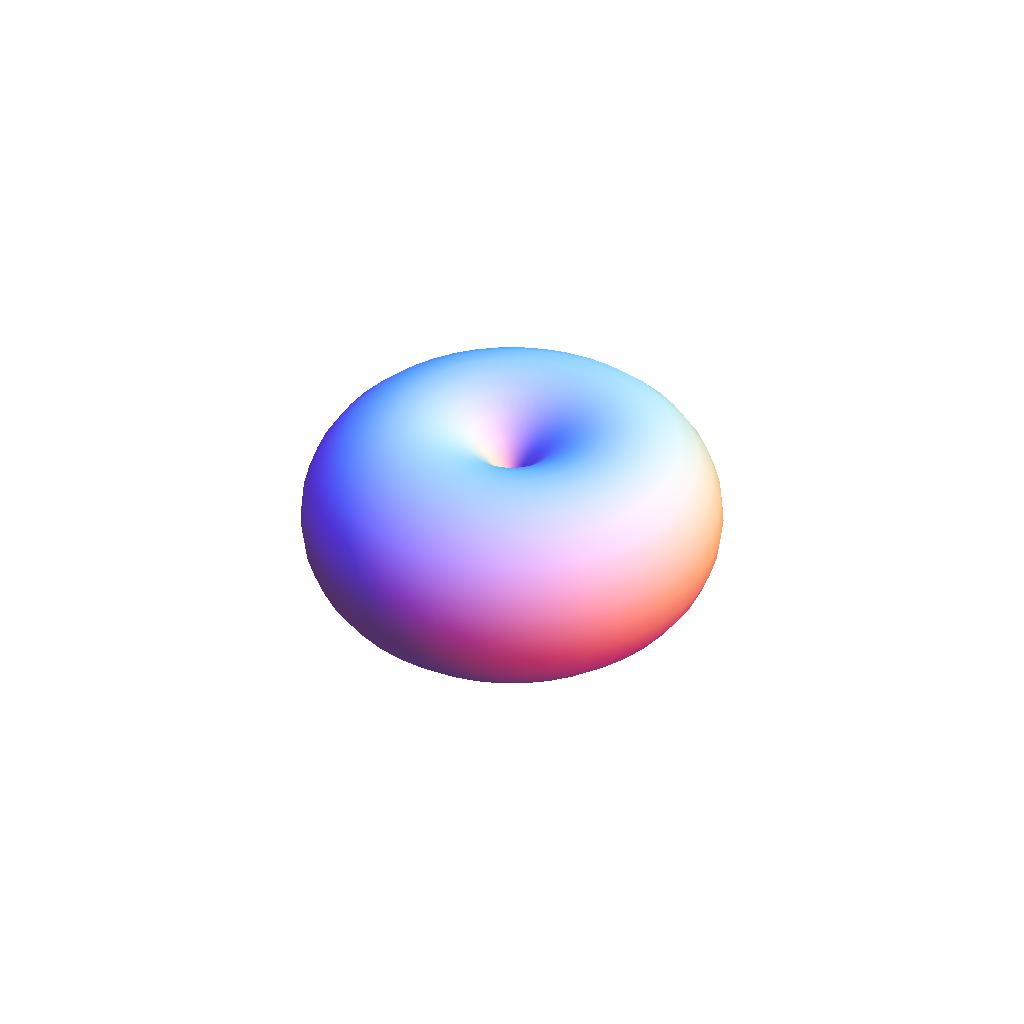
\includegraphics[width= 0.2\textwidth,clip,trim=9cm 8cm 9cm 8cm]{./A06tetel/Y-l1-m1}}
     \\
     \subfloat[$l=2$, $m=0$\label{fig:A06-20}]{
\includegraphics[width= 0.2\textwidth,clip,trim=9cm 5cm 9cm 5cm]{./A06tetel/Y-l2-m0}}
     \hspace{6pt}
     \subfloat[$l=2$, $m=1$\label{fig:A06-21}]{
\includegraphics[width= 0.2\textwidth,clip,trim=9cm 5cm 9cm 5cm]{./A06tetel/Y-l2-m1}}
     \hspace{6pt}
     \subfloat[$l=2$, $m=2$\label{fig:A06-22}]{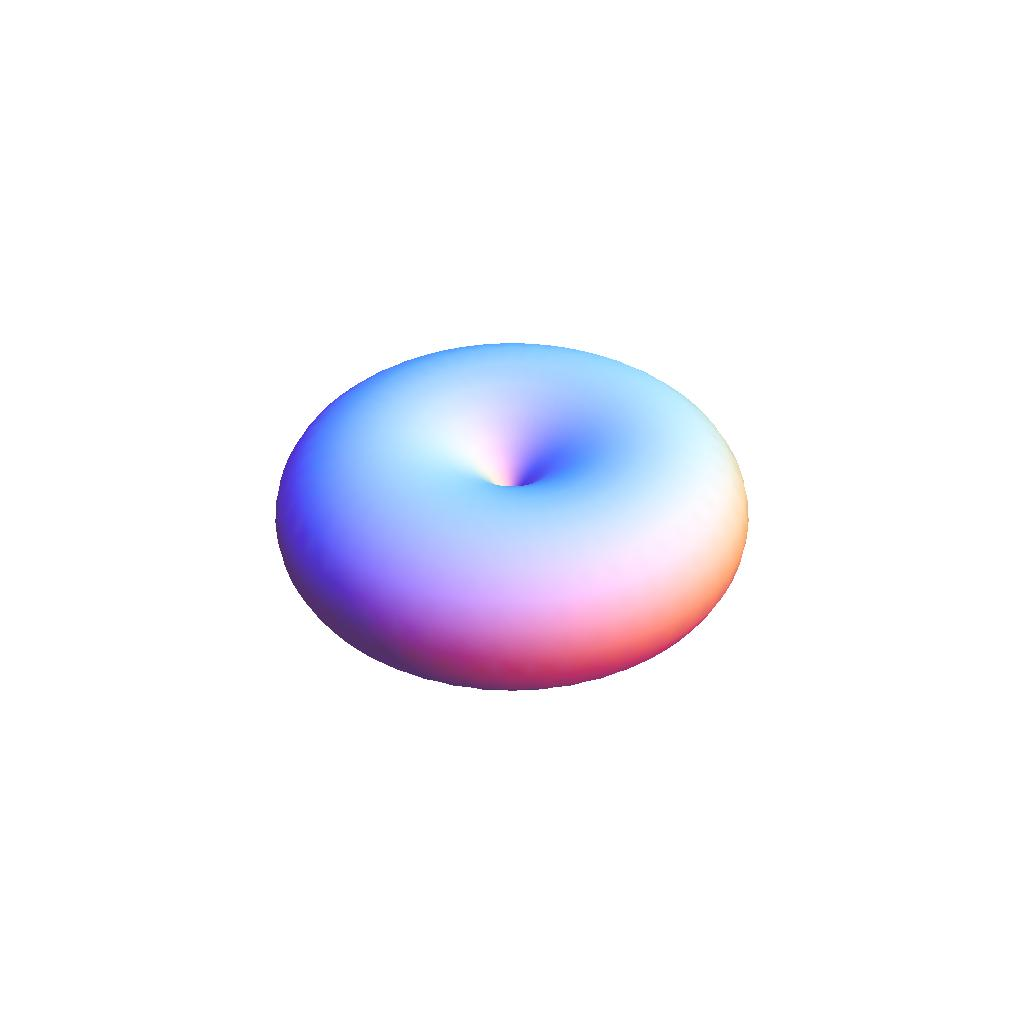
\includegraphics[width= 0.2\textwidth,clip,trim=9cm 5cm 9cm 5cm]{./A06tetel/Y-l2-m2}}
     \\
     \subfloat[$l=3$, $m=0$\label{fig:A06-30}]{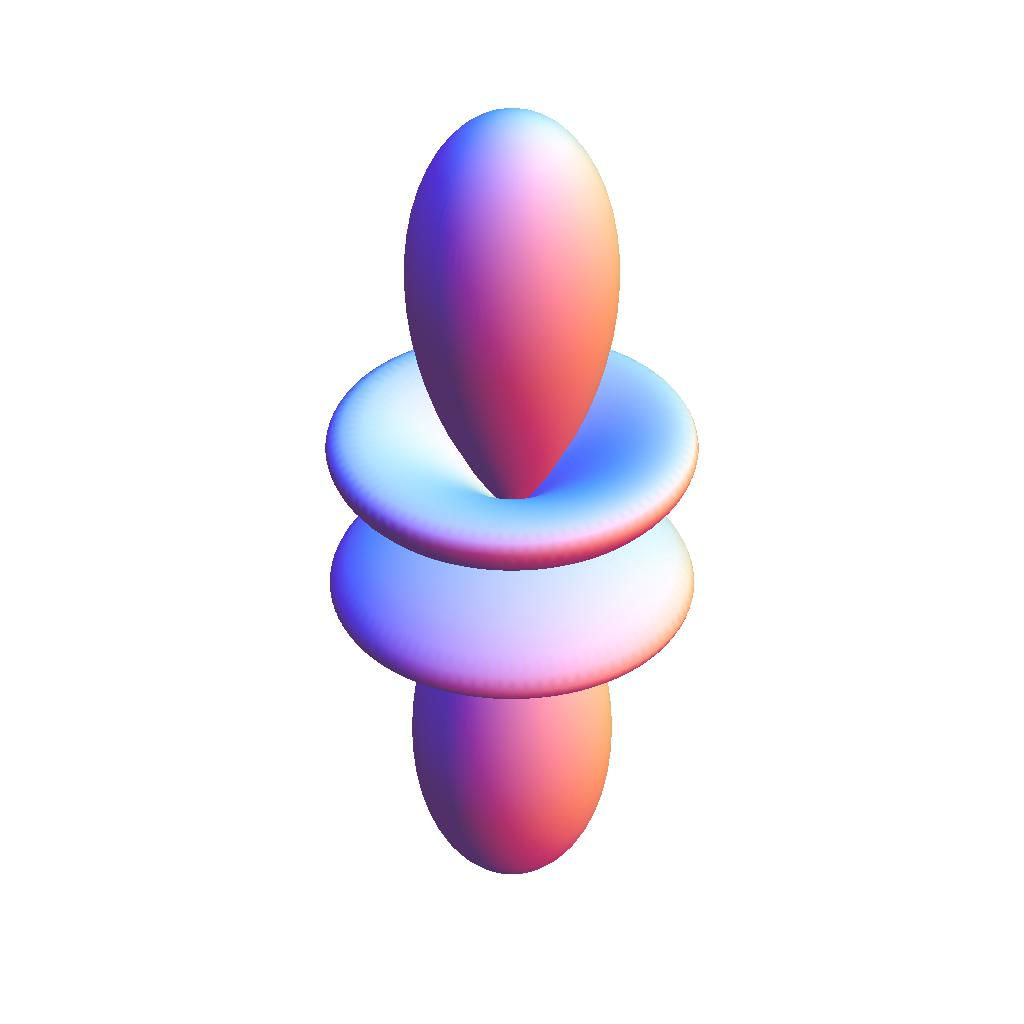
\includegraphics[width= 0.2\textwidth,clip,trim=9cm 3cm 9cm 3cm]{./A06tetel/Y-l3-m0}}
     \hspace{6pt}
     \subfloat[$l=3$, $m=1$\label{fig:A06-31}]{
\includegraphics[width= 0.2\textwidth,clip,trim=9cm 3cm 9cm 3cm]{./A06tetel/Y-l3-m1}}
     \hspace{6pt}
     \subfloat[$l=3$, $m=2$\label{fig:A06-32}]{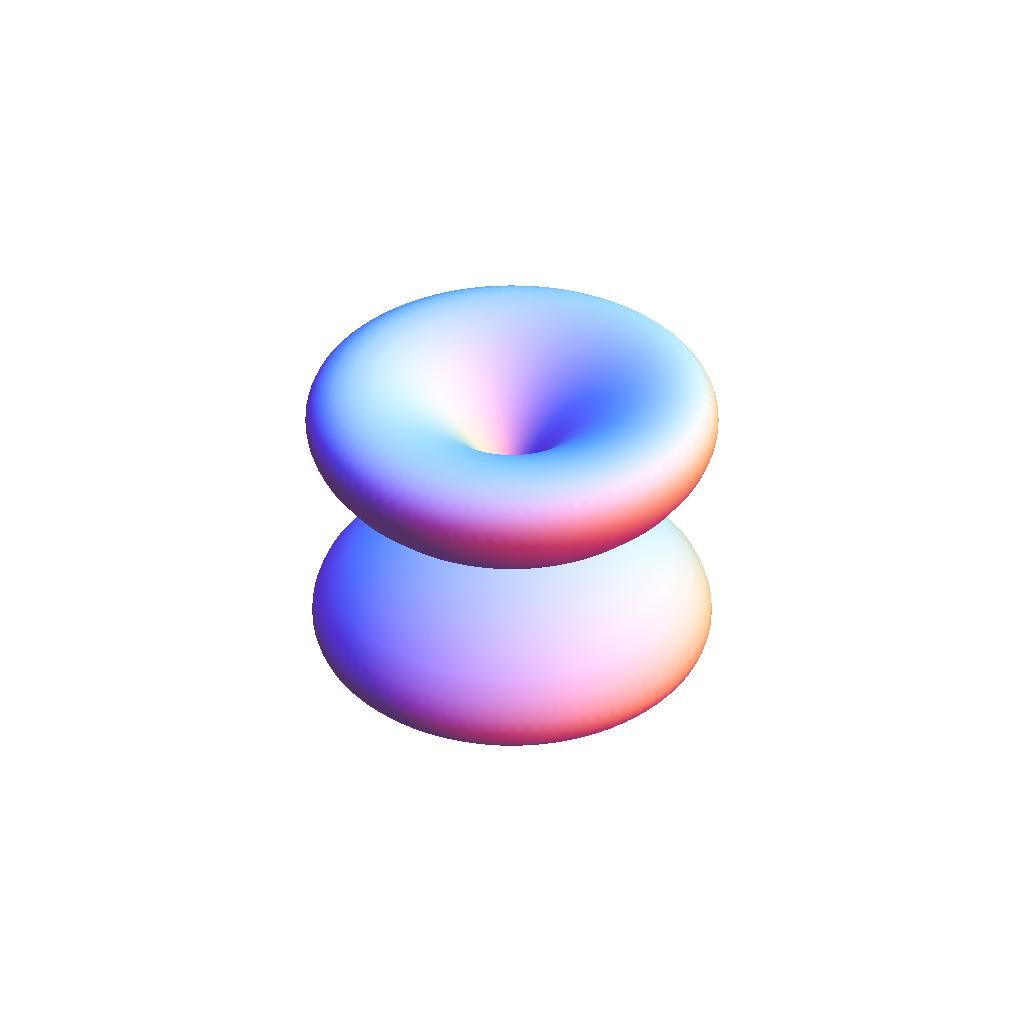
\includegraphics[width= 0.2\textwidth,clip,trim=9cm 3cm 9cm 3cm]{./A06tetel/Y-l3-m2}}
     \hspace{6pt}
     \subfloat[$l=3$, $m=3$\label{fig:A06-33}]{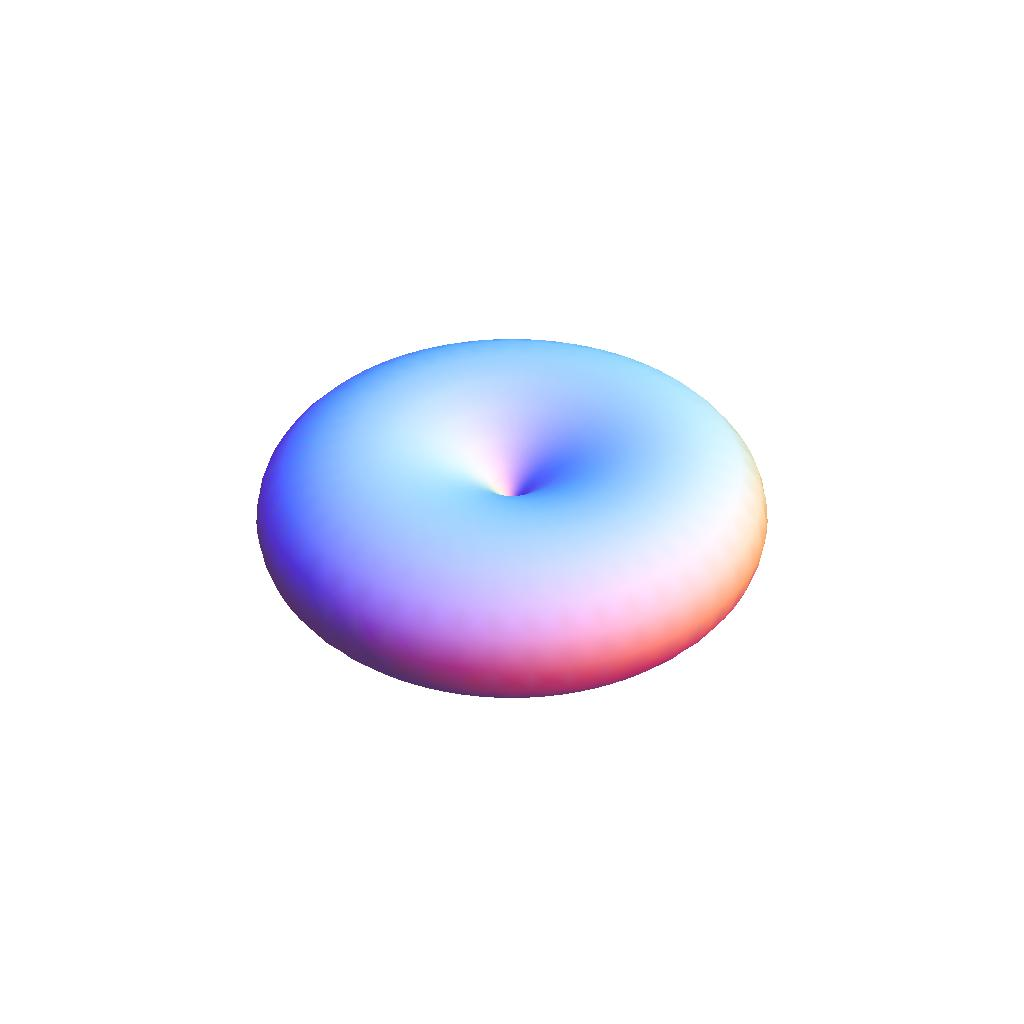
\includegraphics[width= 0.2\textwidth,clip,trim=9cm 3cm 9cm 3cm]{./A06tetel/Y-l3-m3}}
     \\
     \caption{Gömbharmonikusok abszolútértéke ($\abs{Y_l^m(\vartheta,\varphi)}$). (Az ábrák egymáshoz képest méretarányosak.)}
    \end{figure}
% 
%   WIKIPÉDIÁS KONVENCIÓ, nekem jobban tetszik, de Szunyinál a másik van.
%      A Legendre-polinomok:
%      \al{
%       P_l(\cos\vartheta)
%        = \frac{1}{2^l l!} \frac{\dd^l}{\dd (\cos\vartheta)^l} \left[ (\cos^2\vartheta -1)^l \right],
%      }
%      amelyekkel az asszociált Legendre-polinomok:
%      \al{
%       P_l^m (\cos\vartheta)
%        &=(-1)^m \sin^{m}(\cos\vartheta)\frac{\dd^{\abs{m}}}{\dd (\cos\vartheta)^{\abs{m}}}P_l(\cos\vartheta) 
%       &0\le m\le l\\
%       &P_l^{-m} (\cos\vartheta)
%        =(-1)^m \frac{(l-m)!}{(l+m)!}P_l^m(\cos\vartheta).&
%      }
%      ahol így $m$ értéke már $-l$ és $l$ között lehet.
%      
%      A teljes normált megoldások:
%      \al{
%       &Y_l^m(\vartheta,\varphi)=A_l^{m}P_l^m(\cos\vartheta)\cdot e^{im\varphi},
%       &A_l^{m}=\sqrt{\frac{2l+1}{4\pi}}\sqrt{\frac{(l-m)!}{(l+m)!}},
%      }
%      melyek ortogonalitása:
%      \al{
%       \intl{}{}\dd\Omega\,Y_l^m(Y_{l'}^{m'})^*=\delta_{ll'}\delta_{mm'}.
%      }
%      
%      Az $l$ és az $m$ értékei kötöttek: $\Lambda=l(l+1)$, ahol $l=0,1,2,\dots$ és $m=-l,-l+1,\dots,l-1,l$.
%      
%      Tehát az $\opLv^2$ operátor sajátértékproblémájának megoldása:
%      \\[6pt]
%      \fbox{
%       \addtolength{\linewidth}{-10\fboxsep}%
%       \addtolength{\linewidth}{-5\fboxrule}%
%       \begin{minipage}{\linewidth}
%        \vspace{-14pt}
%        \al{
%         &L^2 Y_l^{m}(\vartheta,\varphi)=\hbar^2 l(l+1)Y_l^{m}(\vartheta,\varphi),\\
%         &Y_l^{m}(\vartheta,\varphi)=A_l^{m}P_l^m(\cos\vartheta)\cdot e^{im\varphi} \\
%         &l=0,1,2,\dots\\
%         &m=-l,-l+1,\dots,0,\dots,l-1,l.
%        }
%       \end{minipage}
%      }
% 
    
    
  \subsection{Az $\op{L}_z$ és az $\opLv^2$ sajátértékproblémája léptetőoperátorokkal}
   
   A következő részben olyan operátor-struktúra sajátérték--sajátvektor problémájával foglalkozunk, amelyre egyedül egy megkötés van, azok a $[\op{L}_i,\op{L}_j]=i\hbar\ep_{ijk}\op{L}_k$ kommutációs relációnak tegyenek eleget. 
   
   A két sajátérték-egyenlet:
   \al{
    &\opLv^2\ket{\Lambda,m }=\hbar^2\Lambda \ket{\Lambda,m }\\
    &\op{L}_z\ket{\Lambda,m }=\hbar m  \ket{\Lambda,m }.
   }
   Mivel az $\opLv^2-\op{L}_z^2=\op{L}_x^2+\op{L}_y^2$ pozitív szemidefinit, így a $\Lambda-m^2\geq0$. 
   
   Vezessük be a léptetőoperátorokat:
   \al{
    \op{L}_\pm=\op{L}_x\pm i\op{L}_y.
   }
   Ezek kommutációs relációi az $\op{L}_x$ és az $\opLv^2$ operátorokkal:
   \al{
    [\op{L}_z,\op{L}_\pm]
     &=[\op{L}_z,\op{L}_x]\pm i[\op{L}_z,\op{L}_y]
      =i\hbar \op{L}_y\pm i(-i\hbar \op{L}_x)
      =\pm\hbar(\op{L}_x\pm i\op{L}_y)=\pm\hbar\op{L}_\pm\\
    [\opLv^2,\op{L}_\pm]
     &=[\opLv^2,\op{L}_x]\pm i[\opLv^2,\op{L}_y]
      =0,
   }
   Tehát:
   \al{
    &\opLv^2\big(\op{L}_\pm\ket{\Lambda,m}\big)=\hbar^2\Lambda \big(\op{L}_\pm\ket{\Lambda,m}\big)\\
    &\op{L}_z\big(\op{L}_\pm\ket{\Lambda,m}\big)=\hbar(m\pm 1) \big(\op{L}_\pm\ket{\Lambda,m}\big),
   }
   Vagyis 
   \al{
    \op{L}_\pm\ket{\Lambda,m}=Q^{\pm}_{\Lambda,m}\ket{\Lambda,m\pm 1}.
   }
   A $Q^{\pm}_{\Lambda,m}$-k nem függetlenek egymástól, hiszen:
   \al{
    Q^{+}_{\Lambda,m}
     =\bra{\Lambda,m+1}\op{L}_+\ket{\Lambda,m}
     =\bra{\Lambda,m}\op{L}_-\ket{\Lambda,m+1}^*
     =(Q^{-}_{\Lambda,m+1})^*.
   }
   Válasszuk a $Q^{\pm}_{\Lambda,m}$ együtthatókat valósnak, akkor 
   \al{
    Q_{\Lambda,m}:=Q^{+}_{\Lambda,m}=Q^{-}_{\Lambda,m+1}.
   }
   Fejtsük ki az $\op{L}_+\op{L}_-$ és az $\op{L}_-\op{L}_+$ operátort:
   \al{
    \op{L}_+\op{L}_-
     &=\big(\op{L}_x+i\op{L}_y\big)\big(\op{L}_x-i\op{L}_y\big)
      =\op{L}_x^2+\op{L}_y^2-i[\op{L}_x,\op{L}_y]
      =\op{L}_x^2+\op{L}_y^2+\hbar\op{L}_z
      =\opLv^2-\op{L}_z^2+\hbar\op{L}_z,\\
    \op{L}_-\op{L}_+
     &=\big(\op{L}_x-i\op{L}_y\big)\big(\op{L}_x+i\op{L}_y\big)
      =\op{L}_x^2+\op{L}_y^2+i[\op{L}_x,\op{L}_y]
      =\op{L}_x^2+\op{L}_y^2-\hbar\op{L}_z
      =\opLv^2-\op{L}_z^2-\hbar\op{L}_z.\\
   }
   Ezek hatása egy báziselemre:
   \aln{
    \op{L}_+\op{L}_-\ket{\Lambda,m}
     &=Q_{\Lambda,m-1}\op{L}_+\ket{\Lambda,m-1}
      =Q_{\Lambda,m-1}^2\ket{\Lambda,m}\nonumber\\
     &=\big(\opLv^2-\op{L}_z^2-\hbar\op{L}_z\big)\ket{\Lambda,m}
      =\hbar^2\big(\Lambda-m^2+m\big)\ket{\Lambda,m},\label{eq:06-pm}\\
    \op{L}_-\op{L}_+\ket{\Lambda,m}
     &=Q_{\Lambda,m}\op{L}_-\ket{\Lambda,m+1}
      =Q_{\Lambda,m}^2\ket{\Lambda,m}\nonumber\\
     &=\big(\opLv^2-\op{L}_z^2+\hbar\op{L}_z\big)\ket{\Lambda,m}
      =\hbar^2\big(\Lambda-m^2-m\big)\ket{\Lambda,m}\label{eq:06-mp}.
   }
   Mivel $Q^2_{\Lambda,m}$ nemnegatív, ezért $\Lambda\geq m^2-m$ és $\Lambda\geq m^2+m$, vagyis 
   \al{
    \Lambda\geq\abs{m}(1+\abs{m}).
   }
   Innen következik, hogy $m$ korlátos, létezik egy olyan $m_\text{max}$ és $m_\text{min}$, hogy 
   \al{
    &\op{L}_+\ket{\Lambda,m_\text{max}}=\ket{}_0,&
    &\op{L}_-\ket{\Lambda,m_\text{min}}=\ket{}_0.&
   }
   Helyettesítsük be $\ket{\Lambda,m_\text{min}}$-t \eqaref{eq:06-pm}, illetve a $\ket{\Lambda,m_\text{max}}$-t \eqaref{eq:06-mp} egyenletbe. Ekkor: $\Lambda=m_\text{min}^2-m_\text{min}$ és $\Lambda=m_\text{max}^2+m_\text{max}$. Innen következik, hogy 
   \al{
    m_\text{max}^2+m_\text{max}=m_\text{min}^2-m_\text{min}\\
    \big(m_\text{max}+m_\text{min}\big)\big(m_\text{max}-m_\text{min}+1\big)=0.
   } 
   Ennek értelmes megoldása csak a $l:=m_\text{max}=-m_\text{min}$, amivel $\Lambda=l(l+1)$. Mivel $\Lambda$ és $l$ között egyértelmű a kapcsolat, ezért átindexelhetjük a sajátfüggvényeket.
   
   Összefoglalva tehát:
   \\[6pt]
   \fbox{
    \addtolength{\linewidth}{-10\fboxsep}%
    \addtolength{\linewidth}{-5\fboxrule}%
    \begin{minipage}{\linewidth}
     \vspace{-12pt}
     \al{
      \opLv^2\ket{l,m}&=\hbar^2l(l+1)\ket{l,m}\\
      \op{L}_z\ket{l,m}&=\hbar m\ket{l,m}\\
      \op{L}^{\pm}\ket{l,m}&=\hbar\sqrt{l(l+1)-m(m\pm 1)}\ket{l,m\pm 1}\\
      l&=\frac{1}{2},1,\frac{3}{2},2,\dots\\
      m&=-l,-l+1,\dots,l-1,l.
     }
    \end{minipage}
   }
   
  \subsection{Impulzusmomentum-összeadás}
   
   Vizsgáljuk meg azt az esetet, mikor egy kvantum rendszerhez két impulzusmomentum jellegű mennyiség is tartozik. Ezek különböző Hilbert-téren hatnak: $\Lin(\mathbb{H}_1)\ni\opLv'_1$ és $\Lin(\mathbb{H}_2)\ni\opLv'_2$. A rendszer teljes állapotát a $\mathbb{H}_1\otimes\mathbb{H}_2$ tenzorszorzat Hilbert-téren tudjuk reprezentálni. Terjesszük ki az operátorokat erre a térre: 
   \al{
    &\opLv_1\colon\mathbb{H}_1\otimes\mathbb{H}_2\mapsto\mathbb{H}_1\otimes\mathbb{H}_2,\;\opLv_1=\opLv_1'\otimes\text{id}_{\mathbb{H}_2}&
    &\opLv_1\colon\mathbb{H}_1\otimes\mathbb{H}_2\mapsto\mathbb{H}_1\otimes\mathbb{H}_2,\;\opLv_2=\text{id}_{\mathbb{H}_1}\otimes\opLv'_2.&
   }
   A tenzorszorzat Hilbert-téren egy jó bázis az eredeti bázisokból tenzorszorzattal létrehozott új bázis: $\ket{l_1,m_1,l_2,m_2}=\ket{l_1,m_1}\otimes\ket{l_2,m_2}$
   Az $\opLv_1$ és az $\opLv_2$ sajátértékproblémáját már megoldottuk:
   \al{
    \begin{cases}
     \opLv_1^2\ket{l_1,m_1,l_2,m_2}=\hbar^2l_1(l_1+1)\ket{l_1,m_1,l_2,m_2}\\
     \op{L}_{1,z}\ket{l_1,m_1,l_2,m_2}=\hbar m_1\ket{l_1,m_1,l_2,m_2}\\
     \op{L}_1^{\pm}\ket{l_1,m_1,l_2,m_2}=\hbar\sqrt{l_1(l_1+1)-m_1(m_1\pm 1)}\ket{l_1,m_1\pm 1,l_2,m_2}
    \end{cases} \\
    \begin{cases}
     \opLv_2^2\ket{l_1,m_1,l_2,m_2}=\hbar^2l_2(l_2+2)\ket{l_1,m_1,l_2,m_2}\\
     \op{L}_{2,z}\ket{l_1,m_1,l_2,m_2}=\hbar m_2\ket{l_1,m_1,l_2,m_2}\\
     \op{L}_2^{\pm}\ket{l_1,m_1,l_2,m_2}=\hbar\sqrt{l_2(l_2+1)-m_2(m_2\pm 1)}\ket{l_1,m_1,l_2,m_2\pm 1}.
    \end{cases}
   }
   A teljes impulzusmomentum-operátor $\opLv=\opLv_1+\opLv_2=\opLv_1'\otimes\text{id}_{\mathbb{H}_2}+\text{id}_{\mathbb{H}_1}\otimes\opLv'_2$ szintén a megfelelő algebrát elégíti ki:
   \al{
    \big[\op{L}_i,\op{L}_j]
     &=\big[\op{L}_{1,i}+\op{L}_{2,i},\op{L}_{1,j}+\op{L}_{2,j}]
      =\big[\op{L}_{1,i},\op{L}_{1,j}]
       +\underbrace{\big[\op{L}_{1,i},\op{L}_{2,j}]}_{=0}
       +\underbrace{\big[\op{L}_{2,i},\op{L}_{1,j}]}_{=0}
       +\big[\op{L}_{2,i},\op{L}_{2,j}]\\
     &=i\hbar\ep_{ijk}\big(\op{L}_{1,k}+\op{L}_{2,k}\big)
      =i\hbar\ep_{ijk}\op{L}_k,
   }
   így ennek az operátornak a fentiekhez teljesen hasonló a sajátértékproblémája. 
   \al{
    \begin{cases}
     \opLv^2\ket{l,m}=\hbar^2l(l+1)\ket{l,m}\\
     \op{L}_{z}\ket{l,m}=\hbar m\ket{l,m}\\
     \op{L}^{\pm}\ket{l,m}=\hbar\sqrt{l(l+1)-m(m\pm 1)}\ket{l,m\pm 1}
    \end{cases}
   }
   A kérdés, hogy a $\ket{l,m}$ bázis hogyan viszonyul a direkt szorzat bázishoz:
   \eqn{
    \ket{l,m}
     =\suml{m_1,m_2}{}\bra{l_1,m_1,l_2,m_2}\et{l,m}\ket{l_1,m_1,l_2,m_2},\label{eq:06-cg}
   }
   itt az $\bra{l_1,m_1,l_2,m_2}\et{l,m}$ együtthatók a Clebsch--Gordan-együtthatók. A célunk ezek meghatározása. 
   
   Nézzük meg az $\op{L}_z$ hatását egy általános, \eqref{eq:06-cg} egyenletben megadott állapotra:
   \al{
    \op{L}_z\ket{l,m}
     &=\hbar m \ket{l,m}\\
     &=\suml{m_1,m_2}{}\hbar m\bra{l_1,m_1,l_2,m_2}\et{l,m}\ket{l_1,m_1,l_2,m_2}\\
    \big(\op{L}_{1,z}+\op{L}_{2,z}\big)\ket{l,m}
     &=\big(\op{L}_{1,z}+\op{L}_{2,z}\big)\suml{m_1,m_2}{}\bra{l_1,m_1,l_2,m_2}\et{l,m}\ket{l_1,m_1,l_2,m_2}\\
      &=\suml{m_1,m_2}{}\hbar\big(m_1+m_2\big)\bra{l_1,m_1,l_2,m_2}\et{l,m}\ket{l_1,m_1,l_2,m_2},
   }
   a két összefüggés egyenlőségéből pedig:
   \al{
    0=\suml{m_1,m_2}{}\hbar\big(m_1+m_2-m\big)\bra{l_1,m_1,l_2,m_2}\et{l,m}\ket{l_1,m_1,l_2,m_2}.
   }
   Mivel $\ket{l_1,m_1,l_2,m_2}$ egy teljes rendszer, ez csak úgy lehetséges, ha az együtthatók eltűnnek: $\big(m_1+m_2-m\big)\bra{l_1,m_1,l_2,m_2}\et{l,m}=0$, vagyis
   \eq{
    \boxed{m=m_1+m_2,}
   }
   különben $\bra{l_1,m_1,l_2,m_2}\et{l,m}=0$.
   
   Innen az is következik, hogy $l$ maximálisan $l_\text{max}=l_1+l_1$ lehet. A Clebsch--Gor\-dan-egy\-ütt\-ha\-tók meghatározásához szükségünk lesz az egyik együttható ismeretére. Ehhez először fejtsük ki az $\opLv^2$ operátort a léptető és az $\opL_z$ operátorokkal:
   \al{
    \op{L}_1^{+}\op{L}_2^{-}+\op{L}_1^{-}\op{L}_2^{+}
     &=
       \big(\op{L}_{1,x}+i\op{L}_{1,y}\big)
       \big(\op{L}_{2,x}-i\op{L}_{2,y}\big)
       +
       \big(\op{L}_{1,x}-i\op{L}_{1,y}\big)
       \big(\op{L}_{2,x}+i\op{L}_{2,y}\big)\\
     &=2\big(\op{L}_{1,x}\op{L}_{2,x}+\op{L}_{1,y}\op{L}_{2,y}\big),
   }
   így
   \al{
    \opLv^2
     &=\big(\opLv_1+\opLv_2\big)^2
      =\opLv_1^2+\opLv_2^2+2\opLv_1\opLv_2
      =\opLv_1^2+\opLv_2^2+2\big(\op{L}_{1,x}\op{L}_{2,x}+\op{L}_{1,y}\op{L}_{2,y}+\op{L}_{1,z}\op{L}_{2,z}\big)\\
     &=\opLv_1^2+\opLv_2^2+2\op{L}_{1,z}\op{L}_{2,z}+\op{L}_1^{+}\op{L}_2^{-}+\op{L}_1^{-}\op{L}_2^{+}
   }
   Ennek a hatása egy direkt szorzat Hilbert-tér elemre:
   \al{
    \opLv^2\ket{l_1,m_1,l_2,m_2}
     &=\hbar^2\Big[l_1(l_1+1)+l_2(l_2+1)+2m_1m_2\Big]\ket{l_1,m_1,l_2,m_2}\\
     &\quad+\hbar^2\sqrt{l_1(l_1+1)-m(m_1+ 1)}\sqrt{l_2(l_2+1)-m_2(m_2- 1)}\ket{l_1,m_1+1,l_2,m_2-1}\\
     &\quad+\hbar^2\sqrt{l_1(l_1+1)-m(m_1- 1)}\sqrt{l_2(l_2+1)-m_2(m_2+ 1)}\ket{l_1,m_1-1,l_2,m_2+1}.
   } 
   Vegyünk egy speciális báziselemet: $\ket{l_1,m_1,l_2,m_2}\to\ket{l_1,l_1,l_2,l_2}$. Erre a léptetők nullát adnak, így:
   \al{
    \opLv^2\ket{l_1,l_1,l_2,l_2}
     &=\hbar^2\Big[l_1(l_1+1)+l_2(l_2+1)+2l_1l_2\Big]\ket{l_1,l_1,l_2,l_2}\\
     &=\hbar^2\Big[(l_1+l_2)(l_1+l_2+1)\Big]\ket{l_1,l_1,l_2,l_2},
   }
   illetve
   \al{
    \op{L}_z\ket{l_1,l_1,l_2,l_2}
     &=\big(\op{L}_{1,z}+\op{L}_{2,z}\big)\ket{l_1,l_1,l_2,l_2}
     =\hbar\Big[l_1+l_2\Big]\ket{l_1,l_1,l_2,l_2}.
   }
   Láthatjuk, hogy az $\opLv^2$ és az $\op{L}_z$ úgy hat az $\ket{l_1,l_1,l_2,l_2}$ báziselemen, mintha az a saját $\ket{l_1+l_2,l_1+l_2}$ báziseleme lenne. Ha az operátorok nem látnak különbséget a báziselemek között, akkor azok megkülönböztethetetlenek, vagyis ugyanazok: $\ket{l_1+l_2,l_1+l_2}=\ket{l_1,l_1,l_2,l_2}$, így
   \eq{
    \bra{l_1,l_1,l_2,l_2}\et{l_1+l_2,l_1+l_2}=1.
   }
   
   A többi Clebsch--Gordan-együtthatót a léptetőoperátorok segítségével tudjuk elkészíteni. A léptetés során ki kell használni az egyes báziselemek ortonormáltságát is. 
   
   A kérdés, hogy $l$ milyen értékeket járhat be. Ennek meghatározásához figyelembe kell venni azt, hogy a bázisok elemszáma azonos: $\dim(\mathbb{H}_1)=2l_1+1$, $\dim(\mathbb{H}_2)=2l_2+1$ és $\dim(\mathbb{H}_1\otimes\mathbb{H}_2)=\suml{l=l_\text{min}}{l_\text{max}}(2l+1)$, illetve a direkt szorzat tulajdonságai miatt:
   \al{
    (2l_1+1)(2l_2+1)
     &=\suml{l=l_\text{min}}{l_\text{max}}(2l+1)
      =l_\text{max}(l_\text{max}-1)-l_\text{min}(l_\text{min}-1)+l_\text{max}-l_\text{min}+1\\
     &=l_\text{max}^2+2l_\text{max}-l_\text{min}^2+1
      =(l_1+l_2)^2+2(l_1+l_2)-l_\text{min}^2+1\\
    l_\text{min}^2
     &=\abs{l_1-l_2}.
   } 
   Összefoglalva tehát: $l=l_1+l_2,l_1+l_2-1,\dots,\abs{l_1-l_2}$, $m=m_1+m_2$. 
   
   A Clebsch--Gordan-együtthatók ortonormáltak:
   \eq{
    \suml{m_1,m_2}{}\bra{l_1,m_1,l_2,m_2}\et{l,m}\bra{l_1,m_1,l_2,m_2}\et{l',m'}
     =\delta_{l,l'}\delta_{m,m'},
   }
   illetve teljes rendszert alkotnak:
   \eq{
    \suml{l=\abs{l_1-l_2}}{l_1+l_2}\suml{m=-l}{l}\bra{l_1,m_1,l_2,m_2}\et{l,m}\bra{l_1,m_1',l_2,m_2'}\et{l,m}
     =\delta_{m_1,m_1'}\delta_{m_2,m_2'}.
   }
   
  \subsection{A mágneses momentum és az impulzusmomentum kapcsolata}
   
   Az A-3. tételben láttuk, hogy a Hamilton-operátor mágneses tér jelenlétében
   \al{
   \op{H}=-\frac{\hbar^2}{2m}\Delta+q\phi+\mu_\text{B}\frac{1}{\hbar}\op{\vect{L}}\vect{B} +\frac{q^2B^2}{8m}\vect{r}_\perp^2.
   }
   A 3. tagból, leolvashatjuk mágnese momentum értékét:
   \eq{
    \opmuv_l=-\pder{\op{H}}{\Bv}=-\mu_\text{B}\frac{1}{\hbar}\op\Lv.
   }
   
  \subsection{A spin létezésére utaló kísérletek: Stern--Gerlach-kísérlet}
   
   A Stern--Gerlach-kísérlet során inhomogén mágneses téren keresztül bocsátanak egy ezüstatomokból álló nyalábot. Az ernyőn két részre oszlik a becsapódások helye. Az eredmény a pályamomentummal nem magyarázható, hiszen az ezüst atomok elektronszerkezete: $[\text{Kr}]\;4\text{d}^{10}\;5\text{s}^1$, vagyis a teljes atom pályamomentuma $L=0$. 
   
   A lehetséges magyarázat, hogy az elektron rendelkezik egy saját impulzusmomentummal, így mágneses momentummal ($\muv_s$) is. Ekkor a mágneses térben a potenciális energia: $V=-\muv_s \Bv$. Ha $\Bv(\rv)$ inhomogén (pl. a $z$ irányban), akkor az ezüst atomokra erő hat: $\Fv=-\grad{V}=\mu_{s,z}\der{B}{z}$. A mérés alapján $\mu_{s,z}=\mp\mu_\text{B}$, így jó választás az előzőek alapján $m_s=\pm\frac{1}{2}$, mellyel
   \eq{
    \opmuv_s=-2\mu_\text{B}\frac{1}{\hbar}\opSv.
   }
   
  \subsection{Spin a klasszikus kvantummechanikában}
   
   A spin operátora és a spinállapotok egy a korábbi leírásban szereplő Hilbert-tértől független térhez tartoznak. A feles spin operátorainak legkisebb ábrázolása $2\times2$-esek. A Hilbert-tér bázisának az $\opS_z$ operátor két sajátértékét választjuk: $\ket{\uparrow}$ és $\ket{\downarrow}$.  Ezen a bázison az operátorok a Pauli-mátrixokkal kifejezhetőek: 
   \eq{
    \opSv=\frac{\hbar}{2}\opsigv.
   }
   
   A teljes rendszer hullámfüggvényét a térszerű Hilbert-tér és a spin Hilbert-tér direkt szorzatán adhatjuk meg: 
   \eq{
    \Psi(\rv t;\sigma)=\Psi_\uparrow(\rv t)\alpha+\Psi_\downarrow(\rv t)\beta,
   }
   ahol $\alpha=\bra{\uparrow}\et{s}$ és $\beta=\bra{\downarrow}\et{s}$.
   
   A teljes hullámfüggvényre $z$ irányú mágnese térben a Pauli--Schrödinger-egyenlet igaz:
   \eqn{
    i\hbar\pder{}{t}
    \begin{pmatrix}
     \Psi_\uparrow(\rv t) \\
     \Psi_\downarrow(\rv t)
    \end{pmatrix}
   =\begin{pmatrix}
     \frac{\oppv^2}{2m}+V(\rv)-\mu_\text{B}B\left(i\pder{}{\phi}-1\right)\\
     \frac{\oppv^2}{2m}+V(\rv)-\mu_\text{B}B\left(i\pder{}{\phi}+1\right)
    \end{pmatrix}
    \begin{pmatrix}
     \Psi_\uparrow(\rv t) \\
     \Psi_\downarrow(\rv t)
    \end{pmatrix}.\label{eq:06-PSE}
   }
   
  \subsection{Spin a relativisztikus kvantummechanikában}
   
   Relativisztikusan a spin nem jó kvantumszám, így az önmagában nem értelmezett mennyiség. Kisenergiás határesetben azonban vissza kell kapnunk a fenti összefüggéseket és a fenti értelmezést. 
   
   A stacionárius Dirac-egyenlet (\eqref{eq:02-DE} egyenlet alapján):
   \eq{
    \big[c\vects{\alpha}\opkv+q\phi+mc^2\beta\big]\psi(\minv{x})=E\psi(\minv{x}).
   }
   
   Vegyük fel a négykomponensű $\psi(\minv{x})$ hullámfüggvényeket kétszer kétkomponensű alakban: 
   $\psi(\minv{x})=\begin{pmatrix}
                    \chi(\minv{x})\\
                    \varphi(\minv{x})
                   \end{pmatrix}$,
   mellyel az előző összefüggés mátrixos alakban:
   \eq{
    \begin{pmatrix}
     E-mc^2-q\phi & -c\opsigv\opkv \\
     -c\opsigv\opkv & E+mc^2-q\phi
    \end{pmatrix}
    \begin{pmatrix}
     \chi(\minv{x})\\
     \varphi(\minv{x})
    \end{pmatrix}=
    0
   }
   A második egyenletből fejezzük ki a nagykomponenst: $\chi(\minv{x})=(E+mc^2-q\phi)^{-1}\phi(\minv{x})$, ahol közelítsük az első tagot kis energiákra $2mc^2$-tel. Ezt az első egyenletbe helyettesítve:
   \al{
    0
     &=\big(E-mc^2-q\phi-c\opsigv\opkv\frac{1}{2mc^2}c\opsigv\opkv\big)\chi(\rv t)
      =\left[E-mc^2-q\phi-\frac{1}{2m}\big(\opkv^2+i(\opkv\times\opkv)\opsigv\big)\right]\chi(\rv t)\\
     &=\left[E-mc^2-q\phi-\frac{1}{2m}\opkv^2+\frac{\hbar q}{2m}\Bv\opsigv\right]\chi(\rv t)
      =\left[E-mc^2-q\phi-\frac{1}{2m}\opkv^2-\underbrace{\frac{\hbar e}{2m}}_{\mu_\text{B}}\Bv\frac{2}{\hbar}\underbrace{\frac{\hbar}{2}\opsigv}_{\opSv}\right]\chi(\rv t)\\
     &=\left[E-mc^2-q\phi-\frac{1}{2m}\opkv^2-2\mu_\text{B}\Bv\frac{1}{\hbar}\opSv\right]\chi(\rv t)
   }
   megkapjuk a Pauli--Schrödinger-egyenletet. 